\chapter{Other Approaches}
\label{ch:other_approaches}

In this chapter, we present two methods for sparse matrix reordering that seemed to hold promise. These methods were found by myself to be either computationally difficult to scale for large matrices or were found to have some bottlenecks, but nevertheless represent interesting directions for future work.

\section{Graph Reinforcement Learning for Reordering}

As we know that sparse symmetric matrices can be represented as undirected graphs, it seems promising that this representation allows GNNs to naturally capture the local neighborhood relationships that classical ordering heuristics rely on, such as node degree and clustering patterns.

Traditional heuristics like minimum degree ordering make greedy decisions based on limited local information. There has been a few approaches for using machine learning to learn better heuristics, such as the work by \cite{dasgupta_alpha_2023}, which uses CNN and tackle large matrices by partitioning the graph. 

GNNs, however, can propagate information across multiple hops in the graph, enabling each node to consider not just its immediate neighbors but also the broader structural context. It also allows us to have variable sized graphs. This multi-hop reasoning capability allows the network to anticipate how eliminating one node will affect distant parts of the matrix, potentially leading to more effective ordering decisions.

The message-passing architecture of GNNs naturally models the fill-in process during matrix factorization. When a node is eliminated, it creates new connections between its neighbors, which GNNs can represent through their aggregation and update mechanisms. The network can learn to predict these fill-in patterns and make elimination choices that minimize overall structural complexity.

The graph neural network, as shown in Figure \ref{fig:rl_method}, processes the sparse matrix represented as a graph, computing embeddings for each node based on features such as degree, clustering coefficient, and centrality measures. The actor network uses these embeddings to select which node to eliminate next, while the critic network estimates the value of the current state. The agent receives rewards based on the fill-in generated at each step, with penalties for creating new edges and bonuses for efficient elimination patterns.

\begin{figure}[h]
    \centering
    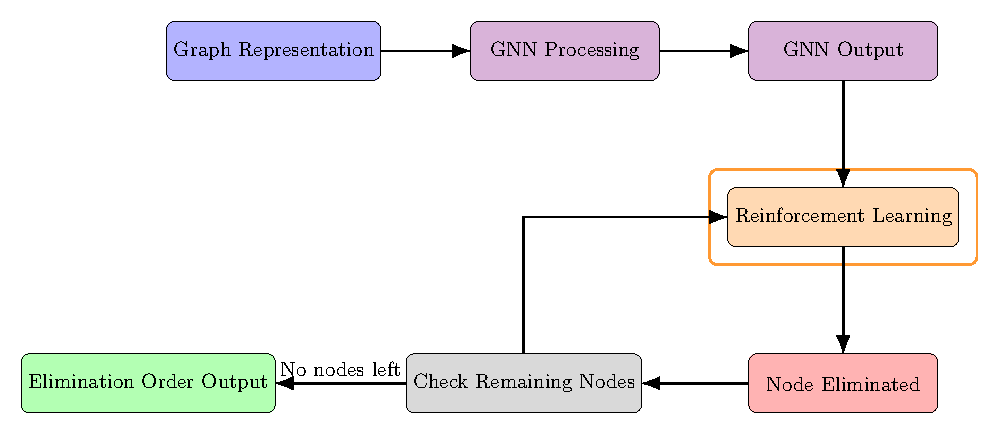
\includegraphics[width=\textwidth]{fig/other/diagram.pdf}
    \caption{Reinforcement Learning Framework for Sparse Matrix Reordering using GNNs}
    \label{fig:rl_method}
\end{figure}

The model shows good and promising results on small matrices, achieving 9.8\% improvement over RCM and 81.4\% improvement over MinDegree on the ash85 matrix, and 28.4\% and 51.0\% improvements respectively on the bcsstk22 matrix. Furthermore, experiments on synthetic graphs with a few hundred nodes demonstrated good results, suggesting the approach can handle moderately sized problems. However, the method struggles to scale to very large matrices due to the computational complexity of training GNNs on large graphs. Future work can explore scaling techniques such as graph coarsening, hierarchical approaches, or coarser representations of the graph to make it feasible for larger matrices.

\section{GPU Accelerated Nested Dissection}

There is very limited work on GPU-accelerated reordering algorithms. I had presented, earlier in this thesis, a GPU implementation of the RCM algorithm. Another promising approach is to implement the nested dissection algorithm on GPUs. One such approach is presented by \cite{yuan_fast_nodate}, which leverages a GPU-based geometry processing library to perform fast graph partitioning, a key step in nested dissection. The method achieves significant speedups over the traditional CPU-based METIS library, but the quality of the ordering is around 3 to 8 times worse than METIS, in their experiments.

\begin{wrapfigure}{l}{0.4\textwidth}
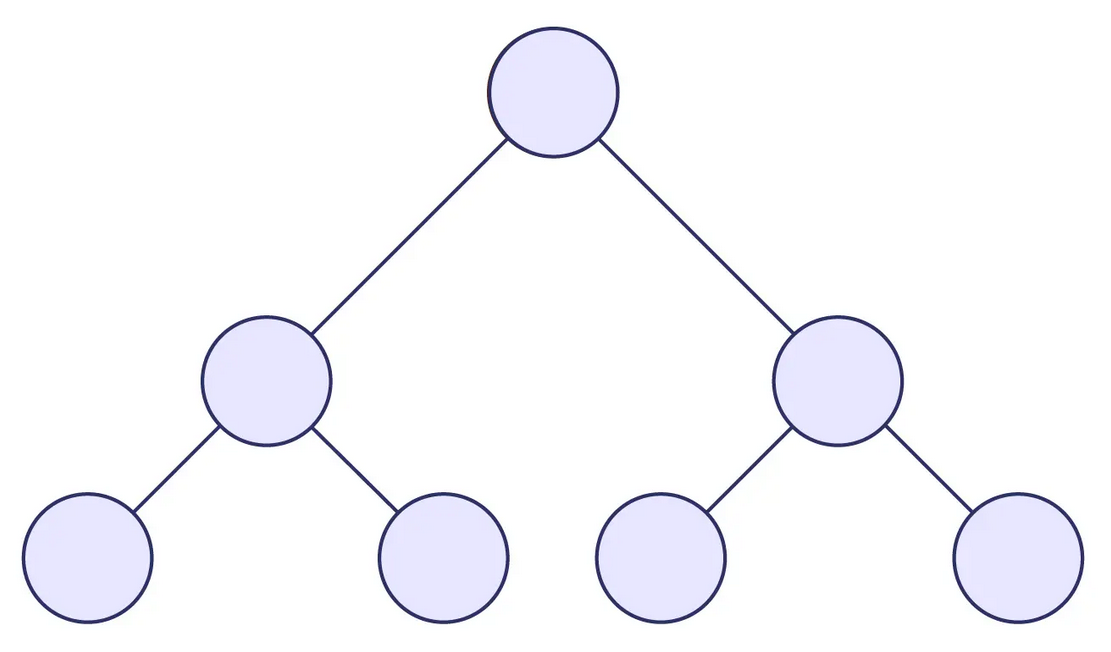
\includegraphics[width=0.9\linewidth]{fig/background/nested_dissection.png} 
\caption{Recursive calls}
\label{fig:nd_res}
\end{wrapfigure}

The primary bottleneck in running nested dissection on GPUs is the recursive nature of the algorithm. Each level of recursion requires partitioning the graph and identifying separators. We leveraged a graph processing library, Jet, which is a multilevel graph partitioning library designed for GPU \cite{gilbert_jet_2024}. The library comes with an efficient implementation of k-way partitioning done using a parallel multilevel approach. One can do a 2-way partitioning by setting k=2, but unsurprisingly, it performs worse in run-time as each call/partition (circle in Figure \ref{fig:nd_res}) is done sequentially. Another approach was to use k = $2^d$, where $d$ is the depth of recursion such each subgraph reaches the threshold size after $d$ levels of recursion. This approach is similar to the approach done using Hypergraph partitioning as mentioned in Chapter \ref{ch:implementation_and_optimizations}, in the way that the partition
divides the graph into smaller subgraphs and the cumulative separators found are placed at the end, producing sparsity-pattern similar to hypergraph based methods in Chapter \ref{ch:implementation_and_optimizations}. This method, which is questionable to call it Nested Dissection, however produces orderings faster than METIS for large graphs but the quality of the ordering is still not comparable to METIS expectedly as you get better separators when you do recursive bisection than a single k-way partitioning. Such an approach produces orderings that are around 2 to 3 times worse than METIS in my experiments on large matrices (\texttt{parabolic_fem.graph} and \texttt{auto.graph}) but the speedups are significant around 5 to 6 times tested on the same environment as mentioned in Chapter \ref{ch:results}.
